\chapter{페르미온, 디랙 행렬, 그리고 디랙 바다}

디랙 바다는 우리가 도달할 곳이지만, 그곳에 이르는 경로도 중요하다. 상대론적 전자 이론에서 음의 에너지를 다루기 전에 두 가지 도구가 필요하다. 먼저 페르미온과 보손을 구분하는 연산자 대수를 살펴본다. 그런 다음 공간 차원이 셋인 기하학적 복잡성 없이 파동함수의 확장을 모두 확인할 수 있는 1차원 디랙 방정식을 복습한다. 이 토대가 갖춰지면 3차원 방정식이 자체적인 행렬 구조를 요구할 것이며, 채워진 페르미온 상태와 비어 있는 페르미온 상태에 관한 앞의 논의는 양전자를 이해하는 열쇠로 다시 등장한다.

\(c=\hbar=1\)를 사용한다. 대문자 \(P\)는 운동량 연산자, 소문자 \(p\)는 운동량 고윳값을 나타내며, 굵은 기호는 이들의 3차원 버전이다.

\section{교환은 연산자 대수가 된다}

서로 구별할 수 없는 두 입자 가운데 하나는 \(x\)에, 다른 하나는 \(y\)에 있다고 하자. \(x\)와 \(y\)은 각각 완전한 위치를 나타낸다. 한 입자의 두 데카르트 좌표를 뜻하는 것이 아니다. 진공에 생성 연산자 두 개를 작용시키면 다음 상태를 얻는다.
\begin{equation}
\lvert x,y\rangle
=
\psi^\dagger(x)\psi^\dagger(y)\lvert0\rangle.
\label{eq:l10-two-particle-state}
\end{equation}

보손의 경우 두 자리를 서로 바꾸어도 상태는 변하지 않는다.
\begin{equation}
\lvert x,y\rangle=\lvert y,x\rangle.
\end{equation}
이 대칭성을 보장하는 연산자 관계는 다음과 같다.
\begin{equation}
\psi^\dagger(x)\psi^\dagger(y)
=
\psi^\dagger(y)\psi^\dagger(x).
\label{eq:l10-boson-exchange}
\end{equation}
보손 생성 연산자 두 개는 서로 가환하므로, 생성되는 상태를 바꾸지 않고 연산자 순서를 뒤집을 수 있다.

페르미온의 경우 교환하면 부호가 바뀐다.
\begin{equation}
\lvert x,y\rangle=-\lvert y,x\rangle.
\label{eq:l10-fermion-state-exchange}
\end{equation}
고립된 상태 벡터의 전체 부호는 관측할 수 없지만, 여러 가능성 사이의 상대적 부호는 관측할 수 있으므로 이 마이너스 부호를 일관되게 유지해야 한다. 식~\eqref{eq:l10-fermion-state-exchange}에 따르면 다음이 성립해야 한다.
\begin{equation}
\psi^\dagger(x)\psi^\dagger(y)
=
-\,\psi^\dagger(y)\psi^\dagger(x).
\label{eq:l10-fermion-operator-exchange}
\end{equation}

\begin{figure}[htbp]\centering
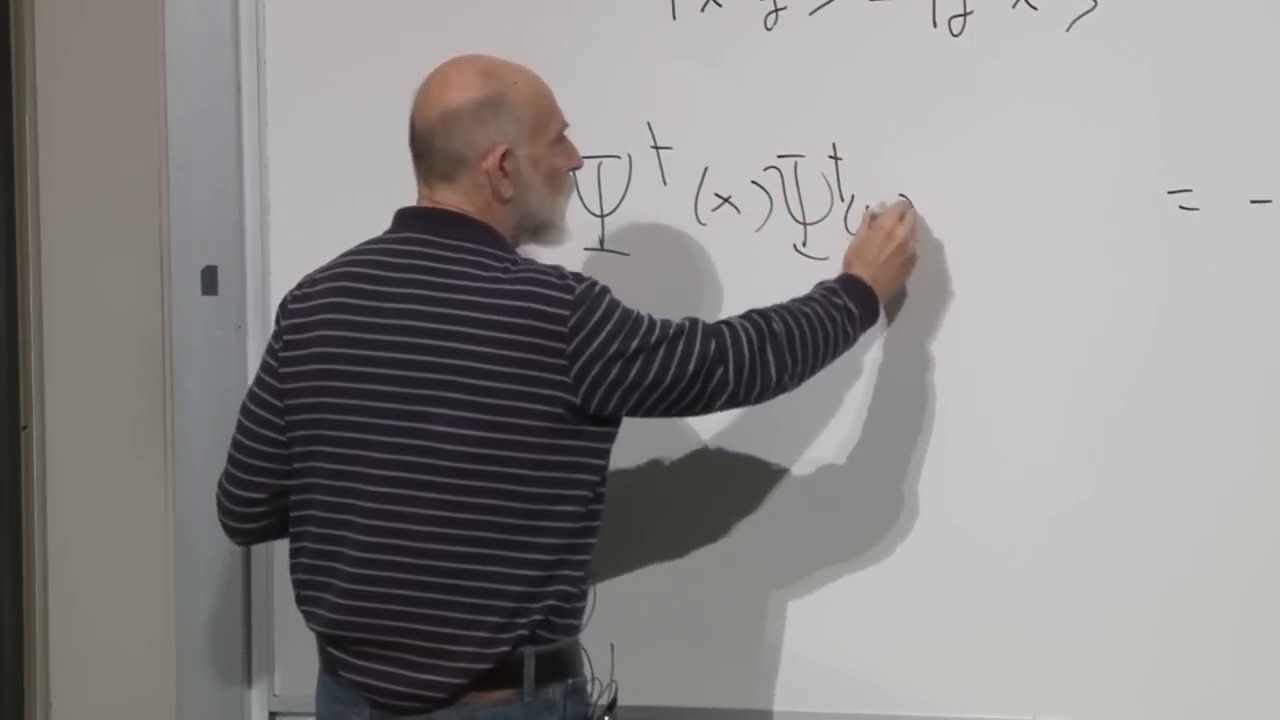
\includegraphics[width=0.94\linewidth]{lecture_10_figure_02.png}\caption{페르미온 교환을 나타내는 칠판 관계. 생성 연산자를 서로 바꾸면 두 입자 상태의 부호가 반전된다.}\lectureframe{00:05:50}\end{figure}

임의의 두 연산자 \(A\)와 \(B\)에 대해 반교환자를 다음과 같이 정의한다.
\begin{equation}
\{A,B\}:=AB+BA.
\end{equation}
따라서 교환 규칙은 다음과 같다.
\begin{equation}
\{\psi^\dagger(x),\psi^\dagger(y)\}=0.
\label{eq:l10-creation-anticommutator}
\end{equation}
이에 대응하는 페르미온 장 대수에서는 보손의 교환자를 반교환자로 바꾼다. 여기서 같은 용어가 두 가지 뜻으로 쓰인다는 점을 구분해야 한다. 장 연산자는 페르미 통계 때문에 서로 반교환하고, 행렬은 뒤에서 상대론적 분산 관계의 교차항을 없애기 위해 서로 반교환한다.

이제 식~\eqref{eq:l10-creation-anticommutator}에서 \(y=x\)로 두자. 두 곱은 서로 같아진다.
\begin{align}
0
&=\{\psi^\dagger(x),\psi^\dagger(x)\}\\
&=2\,\psi^\dagger(x)\psi^\dagger(x).
\end{align}
따라서
\begin{equation}
\bigl(\psi^\dagger(x)\bigr)^2=0.
\label{eq:l10-exclusion}
\end{equation}
동일한 1입자 상태에 동일한 페르미온 두 개를 생성하려 하면 영벡터가 된다. 이것이 연산자 형식으로 쓴 배타 원리다.

\begin{figure}[htbp]
\centering
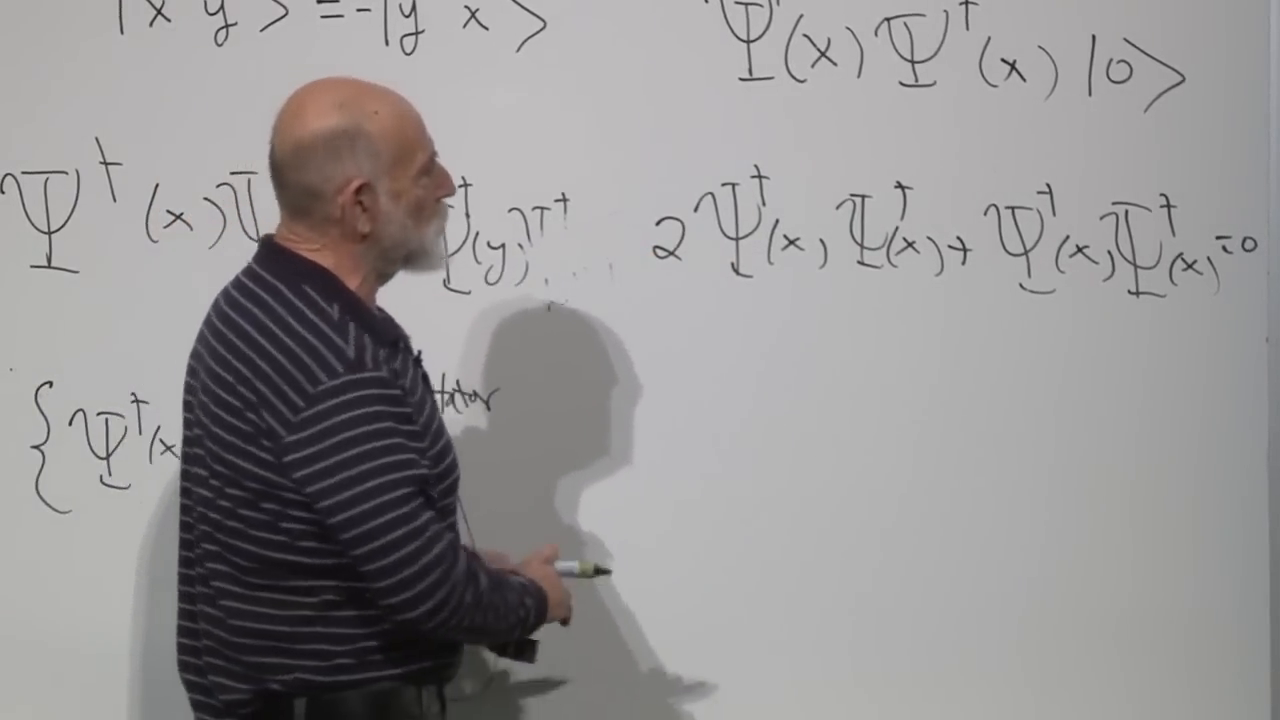
\includegraphics[width=0.94\linewidth]{lecture_10_figure_03.png}
\caption{판서에 나타난 동일 상태의 특수한 경우. 같은 생성 연산자 곱이 두 번 반복되므로 영이 되어야 한다.}
\lectureframe{00:08:04}
\end{figure}

\begin{figure}[htbp]\centering
\begin{adjustbox}{max width=\linewidth}\begin{tikzpicture}[node distance=1.25cm,>=Latex]
\node[draw,rounded corners,align=center,inner sep=7pt] (a)
  {$\{\psi^\dagger(x),\psi^\dagger(x)\}=0$};
\node[draw,rounded corners,align=center,inner sep=7pt,right=of a] (b)
  {$2(\psi^\dagger(x))^2=0$};
\node[draw,rounded corners,align=center,inner sep=7pt,right=of b] (c)
  {$(\psi^\dagger(x))^2=0$};
\draw[->,thick] (a) -- (b);
\draw[->,thick] (b) -- (c);
\end{tikzpicture}\end{adjustbox}\caption{중간의 일부 지워진 칠판 내용을 거치지 않고 다시 구성한 배타 원리 논증.}\end{figure}

\section{페르미온에서 채워짐과 비어 있음이 대칭인 이유}

배타 원리보다 더 미묘하면서 뒤에서 꼭 필요한, 보손 연산자와 페르미온 연산자의 두 번째 차이가 있다. 보손 모드 하나에 대해서는
\begin{equation}
[a,a^\dagger]=1,
\qquad
n=0,1,2,\ldots.
\end{equation}
\(a\)와 \(a^\dagger\)의 순서를 바꾸면 교환자의 부호가 바뀐다. 연산자를 단지 \(A\)와 \(B\)라고 부르더라도, 대수 관계를 보면 어떤 순서가 점유수를 높이고 어떤 순서가 낮추는지 알 수 있다.

보손 점유수 사다리에는 방향도 있다. 소멸 연산자는 결국 \(\lvert0\rangle\)에 도달해 0을 주지만, 생성 연산자는 끝없이 계속 작용할 수 있다.
\begin{align}
a\lvert0\rangle&=0,\\
a^\dagger\lvert n\rangle&\propto\lvert n+1\rangle,
\qquad n=0,1,2,\ldots.
\end{align}
이 사다리를 거꾸로 뒤집는다고 같은 스펙트럼을 얻는 것은 아니다. 아래쪽 끝은 있지만 위쪽 끝은 없다.

페르미온 모드 하나에 대해서는
\begin{equation}
\{a,a^\dagger\}=1,
\qquad
a^2=(a^\dagger)^2=0,
\qquad
n=0,1.
\label{eq:l10-fermion-mode}
\end{equation}
생성 연산자는 빈 상태를 채워진 상태로 바꾼 뒤 더는 작용하지 않는다.
\begin{equation}
a^\dagger\lvert0\rangle=\lvert1\rangle,
\qquad
a^\dagger\lvert1\rangle=0.
\end{equation}
소멸 연산자는 그 반대 작용을 한다.
\begin{equation}
a\lvert1\rangle=\lvert0\rangle,
\qquad
a\lvert0\rangle=0.
\end{equation}
상태가 두 개뿐이므로, 채워진 상태와 빈 상태를 서로 바꾸고 \(a\)와 \(a^\dagger\)를 맞바꾸어도 도식은 대칭이다. 두 연산자의 물리적 의미는 여전히 다르지만, 대수 관계만으로 어느 쪽이 생성이고 어느 쪽이 소멸인지 더는 구별되지 않는다. 이 형식적 대칭성이 입자와 정공의 재해석을 위한 실마리다.

\begin{classroomqa}
\lecturetimestamp{00:13:54}
\audiencequestion{ \((a^\dagger)^2=0\)라면, 모순인가요? 아니면 \(a^\dagger=0\)이라는 뜻인가요?}
\lecturerresponse{둘 다 아닙니다. 0이 아닌 연산자도 제곱이 영일 수 있습니다. 여기서 \(a^\dagger\)은 \(\lvert0\rangle\)을 \(\lvert1\rangle\)로 보내지만, \(\lvert1\rangle\)보다 위에는 허용되는 상태가 없으므로 두 번 적용하면 영이 됩니다. 같은 논리로 \(a^2=0\)도 성립합니다.}
\end{classroomqa}

이 채워짐과 비어 있음의 대칭성을 기억해 두자. 음의 에너지를 가진 전자를 제거할 때 소멸 연산자를 양전자 생성 연산자로 다시 이름 붙이게 된다. 이는 임의로 표기만 바꾸는 것이 아니다. 여기서 확립한 두 상태 페르미온 대수를 그대로 이용하는 것이다.

\section{1차원 디랙 방정식의 구성}

이제 공간 차원이 하나인 곳의 입자 하나로 돌아가자. 가장 간단한 1계 상대론적 파동 방정식은 다음과 같다.
\begin{equation}
i\partial_t\psi=-\,i\partial_x\psi.
\label{eq:l10-right-mover}
\end{equation}
\(P=-i\partial_x\)를 사용하면 이는 다음과 같다.
\begin{equation}
H=P.
\end{equation}
운동량 고유상태에서는 \(E=p\)이고, 군속도는 다음과 같다.
\begin{equation}
v_g=\frac{dE}{dp}=1.
\end{equation}
운동량이 양수든 음수든, 따라서 에너지가 양수든 음수든 파동은 여전히 오른쪽으로 강체 이동한다. \(p\)의 부호는 위상 양상을 바꾸지만 전파 방향은 바꾸지 않는다.

질량이 있는 입자는 양쪽 방향으로 움직일 수 있어야 한다. 다음 조건을 만족하는 두 번째 성분을 도입하자.
\begin{equation}
H\psi_1=P\psi_1,
\qquad
H\psi_2=-P\psi_2.
\label{eq:l10-two-directions}
\end{equation}
첫 번째 성분은 오른쪽으로, 두 번째 성분은 왼쪽으로 움직인다. 이들을 열벡터로 묶고,
\begin{equation}
\Psi=
\begin{pmatrix}
\psi_1\\
\psi_2
\end{pmatrix},
\end{equation}
다음을 정의하면
\begin{equation}
\alpha=
\begin{pmatrix}
1&0\\
0&-1
\end{pmatrix}.
\end{equation}
두 방정식은 모두 다음과 같이 쓸 수 있다.
\begin{equation}
H\Psi=\alpha P\Psi.
\label{eq:l10-massless-one-d}
\end{equation}
양방향을 모두 포함하려면 새로운 2값 내부 자유도가 필요하다.

방향만으로는 질량을 만들 수 없다. 두 번째 행렬을 도입하고,
\begin{equation}
\beta=
\begin{pmatrix}
0&1\\
1&0
\end{pmatrix},
\end{equation}
다음과 같이 놓아 보자.
\begin{equation}
H=\alpha P+\beta m.
\label{eq:l10-massive-one-d}
\end{equation}
행렬들은 다음 관계를 만족한다.
\begin{equation}
\alpha^2=\beta^2=\mathbb{1},
\qquad
\{\alpha,\beta\}=0.
\label{eq:l10-one-d-algebra}
\end{equation}
해밀토니안을 제곱하면 다음을 얻는다.
\begin{align}
H^2
&=(\alpha P+\beta m)^2\\
&=\alpha^2P^2+\beta^2m^2
  +(\alpha\beta+\beta\alpha)Pm\\
&=P^2+m^2.
\label{eq:l10-one-d-dispersion}
\end{align}
식~\eqref{eq:l10-one-d-algebra}의 반교환자 관계 덕분에 \(P\)와 \(m\)에 모두 선형인 원치 않는 항이 사라진다.

비대각 행렬 \(\beta\)는 두 방향 성분을 결합한다. 질량항은 오른쪽 진행 진폭과 왼쪽 진행 진폭을 끊임없이 섞는다고 생각하면 유용하다. 다만 이를 입자가 미시적인 궤도를 따라 앞뒤로 튕겨 다니는 것으로 문자 그대로 받아들여서는 안 된다. 이 그림은 질량이 있는 파동 묶음의 평균 속력이 빛의 속도보다 작을 수 있고 정지계를 가질 수 있는 반면, 고립된 질량 없는 카이랄 성분은 그럴 수 없는 이유를 이해하는 데 도움이 된다.

\begin{classroomqa}\lecturetimestamp{00:23:37}\audiencequestion{양쪽 방향 성분을 모두 도입하는 데 더 깊은 물리적 해석이 있습니까?}\lecturerresponse{있다. 다만 3차원에서 더 분명해진다. 지금 단계에서 이 성분들은 서로 반대 방향으로 전파되는 상태를 기술하고 비대각 질량 결합을 허용하는 데 필요한 두 성분일 뿐이다. 이들의 나중 해석은 손잡이성, 즉 카이랄성이다.}\end{classroomqa}

\section{3차원에서 파울리 행렬이 필연적으로 등장한다}

3차원 공간에서 운동량은 벡터다. 따라서 운동량에 선형이고 회전 스칼라인 해밀토니안에는 또 다른 벡터가 필요해 보인다. 이번에는 성분이 행렬인 벡터다.
\begin{equation}
H=\boldsymbol{\alpha}\cdot\mathbf P
=\alpha_xP_x+\alpha_yP_y+\alpha_zP_z.
\label{eq:l10-three-d-ansatz}
\end{equation}

\begin{figure}[htbp]\centering
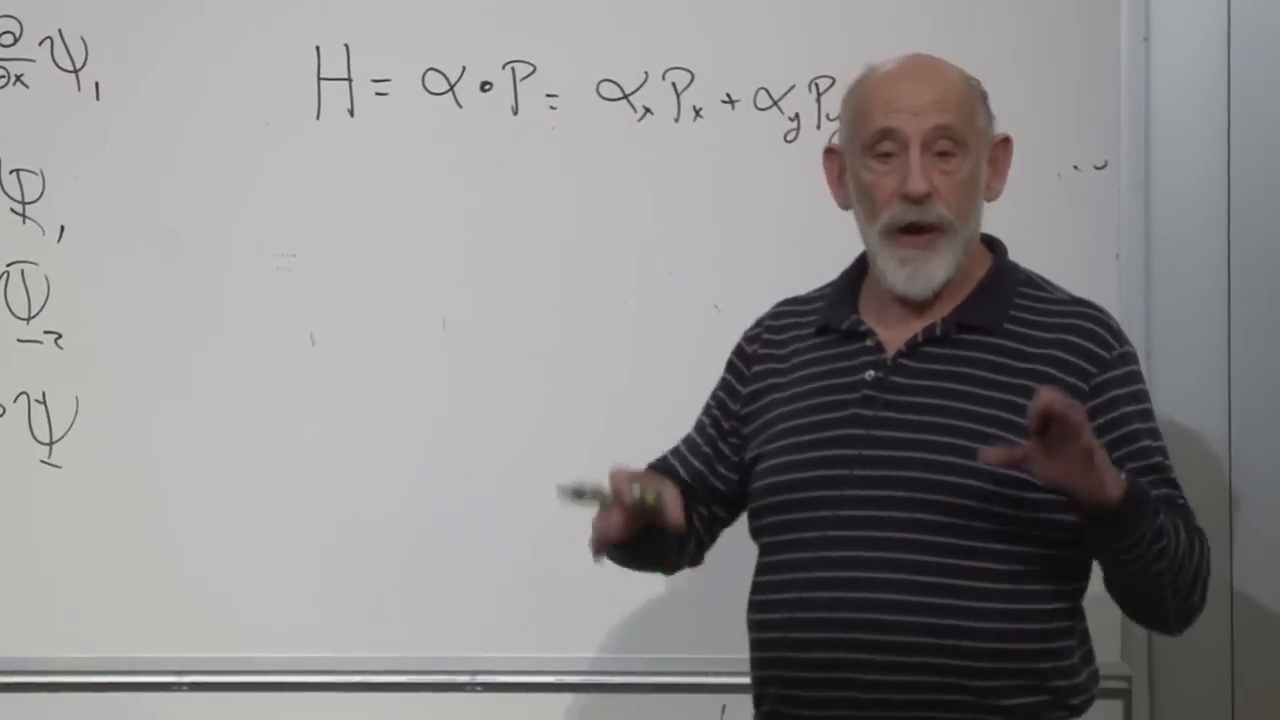
\includegraphics[width=0.94\linewidth]{lecture_10_figure_04.png}\caption{3차원 질량 없는 경우의 가정 \(H=\boldsymbol{\alpha}\cdot\mathbf P\)에서 행렬 하나가 세 행렬의 벡터로 바뀌는 지점.}\lectureframe{00:26:00}\end{figure}

질량 없는 경우부터 다시 시작하자. 다음을 요구한다.
\begin{equation}
H^2=\mathbf P^2=P_x^2+P_y^2+P_z^2.
\end{equation}
식~\eqref{eq:l10-three-d-ansatz}을 제곱해 전개하면
\begin{align}
H^2
&=\alpha_x^2P_x^2+\alpha_y^2P_y^2\\
&\quad+\alpha_z^2P_z^2\\
&\quad+\{\alpha_x,\alpha_y\}P_xP_y\\
&\quad+\{\alpha_x,\alpha_z\}P_xP_z\\
&\quad+\{\alpha_y,\alpha_z\}P_yP_z.
\end{align}
대각항은 다음 조건에서 올바른 값을 갖는다.
\begin{equation}
\alpha_x^2=\alpha_y^2=\alpha_z^2=\mathbb{1},
\end{equation}
모든 교차항이 사라지려면 다음 조건이 필요하다.
\begin{equation}
\{\alpha_i,\alpha_j\}=0,
\qquad i\ne j.
\label{eq:l10-alpha-anticommutation}
\end{equation}

잘 알려진 \(2\times2\) 행렬 세 개가 이 조건을 정확히 만족한다.
\begin{equation}
\sigma_x=
\begin{pmatrix}
0&1\\
1&0
\end{pmatrix},
\quad
\sigma_y=
\begin{pmatrix}
0&-i\\
i&0
\end{pmatrix},
\quad
\sigma_z=
\begin{pmatrix}
1&0\\
0&-1
\end{pmatrix}.
\label{eq:l10-pauli-matrices}
\end{equation}
따라서 한 가지 해는 다음과 같다.
\begin{equation}
\alpha_i=\sigma_i,
\qquad
H=\boldsymbol{\sigma}\cdot\mathbf P.
\label{eq:l10-weyl-hamiltonian}
\end{equation}

\begin{figure}[htbp]\centering
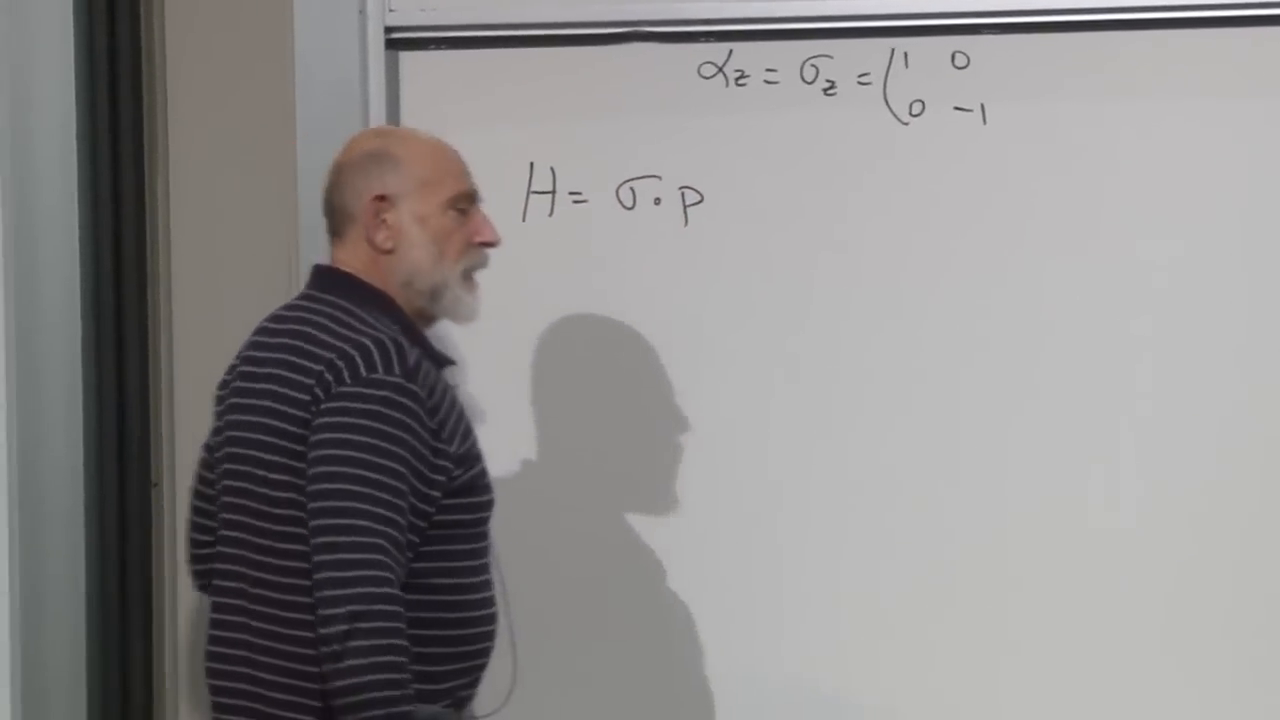
\includegraphics[width=0.94\linewidth]{lecture_10_figure_05.png}\caption{간결한 질량 없는 해밀토니안 \(H=\boldsymbol{\sigma}\cdot\mathbf P\). 그 위에는 \(\alpha_z=\sigma_z\)도 보인다.}\lectureframe{00:28:16}\end{figure}

운동량 고유상태에 대해서는
\begin{equation}
\boldsymbol{\sigma}\cdot\mathbf p
=
|\mathbf p|\,\boldsymbol{\sigma}\cdot\widehat{\mathbf p}.
\end{equation}
연산자 \(\boldsymbol{\sigma}\cdot\widehat{\mathbf p}\)의 고윳값은 \(+1\)과 \(-1\)이므로
\begin{equation}
E=\pm|\mathbf p|.
\end{equation}
이 두 성분 이론에서는 양의 에너지 상태의 파울리 자유도가 운동량과 나란하고, 음의 에너지 상태에서는 반대 방향이다. 이 정렬 관계는 고정된 에너지 부호에서 독립적으로 조절할 수 있는 스핀 방향이 아니다.

\begin{classroomqa}\lecturetimestamp{00:30:10}\audiencequestion{스핀은 디랙 방정식에서 자연히 나오는 것입니까, 아니면 전자가 이미 자기 모멘트를 가진다는 사실을 알고 있었기 때문에 넣은 것입니까?}\lecturerresponse{여기서 자연히 나온다는 것은 사라진다는 뜻이 아니라 결과로서 도출된다는 뜻이다. 출발점은 제곱하면 \(\mathbf P^2\)가 되는, 운동량에 선형인 해밀토니안을 요구하는 것이었다. 보통의 수로는 필요한 대수 관계를 만족시킬 수 없지만 파울리 행렬은 가능하다. 따라서 파울리 행렬의 2성분 구조는 선형화와 함께 등장한다. 그렇다고 모든 입자가 스핀을 가져야 한다는 뜻은 아니다. 이 디랙형 방정식으로 기술되는 입자가 그에 대응하는 스피너 자유도를 가진다는 뜻이다.}\end{classroomqa}

이 구성의 핵심 교훈 가운데 하나다. 상대론적 방정식을 찾은 뒤 행렬을 장식용 표지처럼 덧붙이는 것이 아니다. 상대론적 분산 관계의 국소적인 제곱근을 구하려는 시도에서 행렬이 나온다.

\section{질량에 네 성분이 필요한 이유}

\(2\times2\) 이론을 확장하지 않고 1차원 질량 구성을 반복해 보자:
\begin{equation}
H=\boldsymbol{\sigma}\cdot\mathbf P+\beta m.
\label{eq:l10-failed-mass}
\end{equation}
\(\beta^2=\mathbb{1}\)라고 가정하자. 제곱에는 원하는 항 \(\mathbf P^2+m^2\)이 들어 있지만, 다음 항도 함께 들어 있다.
\begin{equation}
m\sum_i\{\sigma_i,\beta\}P_i.
\end{equation}
이 항을 없애려면 행렬 \(\beta\)은 다음 조건을 만족해야 한다.
\begin{equation}
\{\sigma_x,\beta\}
=
\{\sigma_y,\beta\}
=
\{\sigma_z,\beta\}
=0.
\label{eq:l10-impossible-beta}
\end{equation}
그런 \(2\times2\) 행렬은 없다. 항등행렬은 세 파울리 행렬 모두와 교환하고, 모든 무흔적 \(2\times2\) 행렬은 파울리 행렬들의 선형결합이다. 그런 선형결합은 어느 것이든 그 방향과 평행한 성분과 반교환하지 못한다. \(2\times2\) 대수에는 요구되는 종류의 네 번째 독립 행렬이 없다.

해결책은 스피너를 확장하는 것이다. 제곱하면 항등행렬이 되고 서로 반교환하는 네 행렬은 \(4\times4\) 복소 표현에서 처음 나타난다. 시공간이 네 차원이어서 이 행렬 크기를 택한 것이 아니다. 필요한 대수 구조를 구현할 수 있는 가장 작은 행렬 공간이기 때문이다.

서로 동등한 표현은 여러 가지다. 스피너 기저를 유니터리하게 바꾸면 물리적 예측은 달라지지 않으면서 모든 행렬의 성분이 바뀐다. 중요한 것은 다음과 같은 추상적 관계다.
\begin{equation}
\{\alpha_i,\alpha_j\}=2\delta_{ij}\mathbb{1},
\qquad
\{\alpha_i,\beta\}=0,
\qquad
\beta^2=\mathbb{1}.
\label{eq:l10-dirac-algebra}
\end{equation}

\begin{classroomqa}\lecturetimestamp{00:37:38}\audiencequestion{\(\beta\)를 시간 성분 \(\alpha_t\)로 볼 수 있습니까?}\lecturerresponse{직접 그렇게 볼 수는 없다. 세 \(\alpha_i\)는 \(\beta\)와 함께 하나의 로런츠 벡터를 이루는 네 성분이 아니다. 공변 표기에서는 대신 \(\beta=\gamma^0\)와 \(\alpha_i=\gamma^0\gamma^i\)를 정의하며, 네 \(\gamma^\mu\) 행렬은 시공간 클리퍼드 대수를 만족한다.}\end{classroomqa}

편리한 블록 표현은 다음과 같다.
\begin{equation}
\alpha_i=
\begin{pmatrix}
\sigma_i&0\\
0&-\sigma_i
\end{pmatrix},
\qquad
\beta=
\begin{pmatrix}
0&I_2\\
I_2&0
\end{pmatrix}.
\label{eq:l10-block-representation}
\end{equation}
대각 블록의 파울리 행렬은 서로 다른 \(\alpha_i\)가 반교환하도록 보장한다. \(\beta\)의 비대각 항등행렬 블록은 \(\beta\)가 모든 \(\alpha_i\)와 반교환하도록 보장한다.

\begin{figure}[htbp]\centering
\includegraphics[width=0.94\linewidth]{lecture_10_figure_06.png}\caption{칠판에 적힌 \(4\times4\) 블록 표현. 위의 방정식은 필요한 반교환자 관계를 나타내며, 전체 행렬은 식~\eqref{eq:l10-block-representation}에 적혀 있다.}\lectureframe{00:41:10}\end{figure}

이제 질량이 있는 해밀토니안은 다음과 같다.
\begin{equation}
H=\boldsymbol{\alpha}\cdot\mathbf P+\beta m
=
\begin{pmatrix}
\boldsymbol{\sigma}\cdot\mathbf P&mI_2\\
mI_2&-\boldsymbol{\sigma}\cdot\mathbf P
\end{pmatrix}.
\label{eq:l10-massive-dirac}
\end{equation}
식~\eqref{eq:l10-dirac-algebra}을 사용하면
\begin{equation}
H^2=\mathbf P^2+m^2.
\end{equation}
따라서 네 성분 구조는 선택적으로 덧붙이는 요소가 아니다. 3차원 운동량과 질량항을 모두 포함하면서 방정식을 1계로 유지하는 데 필요한 최소 구조다.

\section{카이랄성과 추가 성분의 의미}

이 확장으로 어떤 물리적 구별이 추가되었을까? 질량 없는 위쪽 블록부터 보자.
\begin{equation}
H_R=\boldsymbol{\sigma}\cdot\mathbf P,
\end{equation}
그리고 질량 없는 아래쪽 블록은
\begin{equation}
H_L=-\boldsymbol{\sigma}\cdot\mathbf P.
\end{equation}
양의 에너지 상태에서 첫 번째 블록은 스핀이 운동량과 나란하고, 두 번째 블록은 스핀이 운동량과 반대 방향이다. 두 상태는 헬리시티가 서로 반대다. 질량 없는 이론에서는 빛과 같은 입자를 추월해 스핀을 그대로 둔 채 운동량 방향을 뒤집을 수 있는 관측자가 없으므로, 헬리시티는 올바른 로런츠 변환 아래 불변이다. 따라서 두 블록은 서로 반대인 카이랄 부문을 기술한다.

\begin{classroomqa}\lecturetimestamp{00:41:28}\audiencequestion{1차원에서는 질량을 도입하려면 추가적인 이진 자유도가 필요했습니다. 3차원에서는 이에 대응하는 물리적 구별이 무엇입니까?}\lecturerresponse{스피너의 손잡이성이다. 두 \(2\times2\) 블록은 스핀과 운동량 사이에 서로 반대인 관계를 갖는다. 하나는 오른손잡이이고 다른 하나는 왼손잡이다. \(4\times4\) 이론에는 둘 다 들어 있다.}\end{classroomqa}

식~\eqref{eq:l10-massive-dirac}의 질량항은 비대각이다. 위쪽 블록의 진폭을 아래쪽 블록으로, 또 그 반대로 바꾼다.
\begin{equation}
\beta m
\begin{pmatrix}
\Psi_R\\
\Psi_L
\end{pmatrix}
=
m
\begin{pmatrix}
\Psi_L\\
\Psi_R
\end{pmatrix}.
\end{equation}
따라서 질량은 반대 카이랄성 사이의 결합이다.

\begin{classroomqa}\lecturetimestamp{00:43:58}\audiencequestion{질량 없는 입자는 카이랄성을 바꿀 수 있습니까?}\lecturerresponse{여기 표시한 자유 질량 없는 해밀토니안에서는 바꿀 수 없다. 두 블록이 서로 분리되어 있으므로, 오른손잡이 또는 왼손잡이로 시작한 상태는 그대로 유지된다. 비대각 질량항이 바로 \(m\ne0\)일 때 두 블록을 섞는 항이다.}\end{classroomqa}

이 표현에서 이 용어는 정확하지만, 입자가 두 화살표 사이를 기계적으로 오가는 모습으로 지나치게 해석해서는 안 된다. 물리적 내용은 파동 방정식의 행렬 결합이다.

\begin{classroomqa}\lecturetimestamp{00:44:50}\audiencequestion{이 행렬들은 쿼터니언에 내재해 있습니까?}\lecturerresponse{파울리 행렬은 쿼터니언 단위와 밀접한 관련이 있다. 행렬 \(-i\sigma_i\)는 \(-\mathbb{1}\)의 제곱을 가지며, 방향 규약에 따른 차이를 제외하면 쿼터니언과 같은 곱셈 패턴을 따른다. 전체 디랙 행렬에는 더 큰 클리퍼드 대수가 필요하며, 이어지는 논증에는 쿼터니언과의 관련이 필요하지 않다.}\end{classroomqa}

\begin{classroomqa}\lecturetimestamp{00:46:34}\audiencequestion{스핀이 각운동량이라면, 여기에는 스핀에 해당하는 별도의 에너지 항이 있습니까?}\lecturerresponse{독립적인 자유 입자 항을 추가하는 것은 아니다. 스피너 구조는 행렬을 통해 이미 운동에너지 해밀토니안에 들어 있다. 스핀을 외부 자기장과 결합하면 상호작용 항이 추가되지만, 그것은 별개의 문제다.}\end{classroomqa}

\section{알파 행렬은 스핀이 아니라 속도다}

각 \(\alpha_i\)는 \(+1\)와 \(-1\)의 두 고윳값을 갖는다. 서로 다른 성분은 가환하지 않으므로 모두를 동시에 정확하게 측정할 수는 없다. 한 성분이 무엇을 나타내는지 알아보려면 하이젠베르크 방정식을 사용하자. 시간에 명시적으로 의존하지 않는 연산자 \(L\)에 대해
\begin{equation}
\dot L=i[H,L].
\label{eq:l10-heisenberg}
\end{equation}
여기서는 Schr\"odinger 시간발전 \(e^{-iHt}\)에 따라 부호 규약을 정했다.

식~\eqref{eq:l10-heisenberg}을 위치 연산자 \(x\)에 적용하자. 행렬은 스피너 첨자에 작용하며 위치와 가환하고, \(P_x\)만이 \(x\)와 가환하지 않는다.
\begin{align}
\dot x
&=i[\boldsymbol{\alpha}\cdot\mathbf P+\beta m,x]\\
&=i\alpha_x[P_x,x]\\
&=\alpha_x,
\label{eq:l10-velocity}
\end{align}
이는 \([P_x,x]=-i\)이기 때문이다. 따라서 \(\alpha_x\)는 속도 연산자의 \(x\) 성분이다. 마찬가지로
\begin{equation}
\dot{\mathbf x}=\boldsymbol{\alpha}.
\end{equation}

\begin{classroomqa}\lecturetimestamp{00:51:50}\audiencequestion{속도 성분을 측정하면 정말 \(+1\) 또는 \(-1\)만 나옵니까?}\lecturerresponse{단위 \(c=1\)에서 순간 연산자 \(\alpha_i\)의 경우에는 그렇다. 일반적인 상태는 고유상태일 필요가 없으므로 기댓값은 그 값들 사이의 어떤 값도 될 수 있다. 부드럽게 이동하는 파동 묶음의 평균 속도는 입자에 질량이 있으면 빛의 속도보다 작다.}\end{classroomqa}

속도는 보존되지 않는다.
\begin{equation}
\dot\alpha_x=i[H,\alpha_x]\ne0.
\end{equation}
\(\alpha_y\), \(\alpha_z\), \(\beta\)를 포함하는 항들은 \(\alpha_x\)와 가환하지 않는다. 따라서 양의 에너지 성분과 음의 에너지 성분이 모두 들어 있는 상태의 위치에는 빠르게 진동하는 성분이 나타난다. 이것이 \emph{zitterbewegung}, 즉 문자 그대로 떨림 운동이다.

빠른 진동보다 훨씬 긴 시간에 걸쳐 평균을 내면, 기대되는 상대론적 속도는 다음과 같다.
\begin{equation}
\overline{\mathbf v}=\frac{\mathbf p}{E},
\end{equation}
이는 느린 전자의 경우 \(\mathbf p/m\)로 근사된다.

\begin{classroomqa}\lecturetimestamp{00:54:40}\audiencequestion{외력이 없는데 자유 전자가 떨며 움직인다면 뉴턴 법칙에 어긋납니까?}\lecturerresponse{아니다. 병진 대칭성에 의해 운동량이 보존되므로 \(\dot{\mathbf P}=0\)다. 디랙 속도 연산자는 단순히 \(\mathbf P/m\)가 아니며, 운동량이 고정된 채로도 그 빠른 진동 성분은 변할 수 있다. 시간 평균 운동은 자유 입자에 대해 예상되는 관계를 따른다.}\end{classroomqa}

\begin{classroomqa}\lecturetimestamp{00:55:22}\audiencequestion{속도는 항상 \(c\)입니까?}\lecturerresponse{하나의 \(\alpha_i\)를 순간적으로 측정하면 고윳값은 \(\pm c\)이지만, 질량이 있는 파동 묶음은 일반적으로 중첩 상태이므로 기댓값은 광속보다 작다. 평균 군속도는 \(\mathbf p/E\)이다.}\end{classroomqa}

\begin{classroomqa}\lecturetimestamp{00:55:30}\audiencequestion{진동을 질량이 속도를 변화시키는 것으로 그려도 될까요?}\lecturerresponse{아니다. 질량은 고정된 매개변수다. 진동은 속도 연산자와 해밀토니안 연산자가 가환하지 않기 때문에, 또는 동등하게 에너지 부문 사이의 간섭 때문에 생긴다. 질량이 요동해서 생기는 현상이 아니다.}\end{classroomqa}

\begin{classroomqa}\lecturetimestamp{00:56:22}\audiencequestion{평균 운동 방향은 반대인데도 순간 측정에서는 속도가 한쪽을 가리킬 수 있습니까?}\lecturerresponse{그렇다. 성분 연산자는 두 개의 명확한 고윳값을 가지지만, 반복 측정이나 시간 평균 측정에서는 더 부드러운 표류 운동이 드러난다.}\end{classroomqa}

스핀이라는 용어도 주의해서 써야 한다. \(\alpha_i\)는 일반 벡터인 속도의 성분처럼 변환한다. 이 표현에서 진짜 스핀 연산자는 다음과 같다.
\begin{equation}
\mathbf S=\frac12\boldsymbol{\Sigma},
\qquad
\Sigma_i=
\begin{pmatrix}
\sigma_i&0\\
0&\sigma_i
\end{pmatrix}.
\label{eq:l10-spin-operator}
\end{equation}
이는 아래쪽 블록의 부호가 \(\alpha_i\)와 다르다. 두 행렬은 밀접한 관련이 있지만, 속도와 스핀은 같은 관측량이 아니다.

\section{음의 에너지와 최저 에너지 진공}

음의 에너지 문제는 이 행렬 도구를 도입하기 전부터 이미 존재한다. 1차원 오른쪽 진행파로 돌아가자.
\begin{equation}
H=P.
\end{equation}
\(p\)가 실수 전체를 훑으므로 \(E=p\)는 아래쪽으로 유계가 아니다.

진공은 단순히 입자가 없는 상태를 뜻할 수 없다. 더는 에너지를 꺼낼 수 없는 상태여야 한다. 빈 상태에서 음의 에너지 입자를 더해 에너지를 낮추고, 또 하나를 더하는 일을 끝없이 계속할 수 있다면 그 빈 상태는 안정된 진공이 아니다.

페르미 통계는 역사적으로 이 문제를 해결하는 방법을 제공한다. 음의 에너지 상태마다 전자 하나씩을 놓는다. 전자를 더할 때마다 전체 에너지는 낮아지지만, 배타 원리에 따라 각 1입자 상태에는 전자 하나만 들어갈 수 있다. 음의 에너지 상태가 모두 채워지면 더는 전자가 그 부문으로 떨어져 들어갈 수 없다. 디랙은 이렇게 채워진 구성을 진공으로 보았다.

같은 구성은 보손에는 통하지 않는다. 보손은 한 상태에 얼마든지 들어갈 수 있으므로, 음의 에너지 보손 모드는 한계 없이 입자를 받아들일 수 있다. 강의 앞부분에서 소개한 페르미온의 제한 \(n=0,1\)이 바로 에너지가 계속 내려가는 것을 막는다.

\begin{figure}[htbp]\centering
\includegraphics[width=0.94\linewidth]{lecture_10_figure_07.png}\caption{칠판에 그린 역사적 디랙 바다 그림. 음의 에너지 준위는 경계선까지 채워져 있고 그 위에는 양의 에너지 상태가 놓여 있다.}\lectureframe{01:02:45}\end{figure}

\begin{figure}[htbp]\centering
\begin{adjustbox}{max width=\linewidth}\begin{tikzpicture}[x=1.05cm,y=0.72cm,>=Latex]
\draw[->] (0,-4.8) -- (0,4.8) node[above] {$E$};
\draw[thick] (-2.9,0) -- (3.2,0) node[right] {$E=0$};
\foreach \y in {-4,-3.3,...,-0.5} {
  \draw (-2.3,\y) -- (2.3,\y);
  \foreach \x in {-1.8,-1.2,...,1.8} {
    \fill[blue!65!black] (\x,\y) circle (1.6pt);
  }
}
\foreach \y in {0.8,1.6,...,4.0} {
  \draw (-2.3,\y) -- (2.3,\y);
}
\draw[red,very thick] (0.6,-2.6) circle (5pt);
\draw[red,->,very thick] (0.6,-2.35) .. controls (1.4,-0.4) and (1.2,1.6) .. (1.5,2.4);
\fill[red] (1.5,2.4) circle (2.5pt);
\node[right,red] at (0.85,-2.6) {hole};
\node[right,red] at (1.7,2.4) {$e^-$};
\node[left] at (-2.5,-2.2) {filled negative-energy states};
\end{tikzpicture}\end{adjustbox}\caption{채워진 바다 위의 들뜸을 깔끔하게 다시 그린 그림. 음의 에너지 전자 하나를 높은 에너지 상태로 올리면 양의 에너지 정공이 남는다.}\end{figure}

바다 그림은 올바른 연산자 재배열을 역사적인 표현으로 설명한 것이다. 무한한 전하와 에너지를 문자 그대로의 물리량으로 보아 직접 관측할 수 있다고 오해해서는 안 된다. 현대적 재정식화에서는 물질로 된 전자가 공간을 채운다고 상상할 필요가 없다.

\section{정공은 양전자다}

음의 에너지 상태가 모두 채워져 있으면 두 종류의 들뜸이 가능하다. 바다 위에 양의 에너지 전자를 더할 수 있다. 또는 음의 에너지 전자 하나를 제거해 정공을 남길 수 있다.

정공은 사라진 전자와 반대 전하를 갖는다. 전하 \(-e\)를 제거하면 전하가 \(+e\)만큼 변한다. 정공은 양의 들뜸 에너지도 갖는다. 제거된 전자의 에너지가 \(E_-<0\)였다면, 채워진 진공을 기준으로 잰 에너지 변화는 다음과 같다.
\begin{equation}
E_{\mathrm{hole}}=-E_->0.
\end{equation}
정공은 양의 에너지와 양전하를 가진 들뜸, 즉 양전자다.

광자는 바다의 전자를 양의 에너지 상태로 올릴 수 있다. 진공을 기준으로 보면 최종 상태에는 전자와 양전자가 들어 있다. 시간 순서가 있는 도식에서는 전자 수 흐름을 전자의 경우 위쪽 화살표로, 양전자 선은 반대 화살표로 그리는 것이 관례다. 화살표는 페르미온 수 또는 전하의 흐름을 나타내며, 고전적인 속도 벡터를 작게 그린 것이 아니다.

\begin{classroomqa}\lecturetimestamp{01:05:14}\audiencequestion{이 그림에서는 전자와 양전자의 수가 같아야 합니까?}\lecturerresponse{임의의 상태에 대해서는 그렇지 않다. 진공에서 중성 쌍을 만들면 전자와 양전자가 하나씩 생기지만, 상태에 전자나 양전자가 이미 더 많이 들어 있을 수 있다. 전하 보존은 반응을 제한할 뿐, 허용되는 모든 상태에서 두 입자의 수가 같아야 한다고 요구하지 않는다.}\end{classroomqa}

디랙은 처음에는 정공이 전자와 질량은 같고 전하와 다른 가법적 양자수만 반대인 입자라는 사실을 몰랐다. 디랙 방정식과 정공 구성에서 그런 예측이 나왔으며, 양전자는 익숙한 입자 목록에 포함되기 전에 먼저 이론적으로 예견되었다.

\section{하나의 페르미온 장에 전자와 양전자가 함께 들어 있다}

장 연산자는 역사적 그림을 현대적 대수로 가져온다. 우선 스피너 첨자, 정규화 인자, 시간 의존성을 잠시 생략하자. 1차원 장은 도식적으로 다음과 같이 전개할 수 있다.
\begin{equation}
\psi(x)
\sim
\int_{-\infty}^{\infty}dp\,a(p)e^{ipx}.
\label{eq:l10-full-field-integral}
\end{equation}
오른쪽 진행 분산 관계 \(E=p\)에서 양의 \(p\)는 양의 에너지를, 음의 \(p\)는 음의 에너지를 나타낸다. 적분을 나누면
\begin{equation}
\psi(x)
\sim
\int_0^\infty dp\,a(p)e^{ipx}
+
\int_{-\infty}^0 dp\,a(p)e^{ipx}.
\end{equation}
두 번째 항에서 \(p=-q\)로 치환하면 \(q>0\)이고, 음의 에너지 전자의 소멸을 양전자 생성으로 재해석한다.
\begin{equation}
b^\dagger(q):=a(-q).
\end{equation}
그러면
\begin{equation}
\psi(x)
\sim
\int_0^\infty dp\,
\left[
a(p)e^{ipx}
+
b^\dagger(p)e^{-ipx}
\right].
\label{eq:l10-electron-positron-split}
\end{equation}
평면파 위상의 정확한 부호는 시공간 규약에 따라 달라진다. 불변인 내용은 \(\psi\)에 전자 소멸 연산자와 양전자 생성 연산자가 들어 있다는 것이다.

\begin{figure}[htbp]\centering
\includegraphics[width=0.94\linewidth]{lecture_10_figure_08.png}\caption{양의 에너지 부문과 음의 에너지 부문으로 나눈 장 적분. 아래 줄에서는 음의 에너지 전자 연산자를 양전자 생성 연산자로 다시 이름 붙인다.}\lectureframe{01:11:35}\end{figure}

여기서 식~\eqref{eq:l10-fermion-mode}의 채워짐과 비어 있음의 대칭성이 효과를 발휘한다. 페르미온에서는 반교환 구조를 바꾸지 않고도 연산자를 다시 이름 붙일 수 있다.

전자기 상호작용의 도식적 형태는 다음과 같다.
\begin{equation}
H_{\mathrm{int}}
\sim
\int dx\,\psi^\dagger(x)\psi(x)A(x),
\label{eq:l10-qed-schematic}
\end{equation}
여기서 \(A\)는 광자장을 나타낸다. 각 페르미온 장에 전자와 양전자 성분이 모두 들어 있으므로, 하나의 국소 연산자에 여러 반응 경로가 포함된다.
\begin{align}
e^-&\longrightarrow e^-+\gamma,\\
e^-+e^+&\longrightarrow\gamma,\\
\gamma&\longrightarrow e^-+e^+,
\end{align}
여기에 역반응과 교차 반응도 포함된다. 특정 환경에서 어떤 경로가 운동학적으로 가능한지는 에너지와 운동량 보존이 결정한다. 예를 들어 상호작용 꼭짓점이 있더라도, 진공 속에서 고립된 실재 광자는 반동을 받아줄 다른 입자가 없으면 쌍을 만들 수 없다.

\begin{figure}[htbp]\centering
\includegraphics[width=0.94\linewidth]{lecture_10_figure_09.png}\caption{칠판에는 전자 방출, 쌍소멸, 그리고 도식적 상호작용 \(\psi^\dagger\psi A\)가 함께 그려져 있다. 같은 장 연산자에서 서로 다른 항을 선택하면 각기 다른 반응 경로가 나온다.}\lectureframe{01:13:30}\end{figure}

따라서 장을 간결하게 곱한 하나의 식이 겉보기에는 서로 달라 보이는 여러 반응을 함께 기술한다. 파인만은 나중에 진폭을 계산하기 위한 체계적인 도식 규칙을 제시했지만, 연산자 구조의 많은 부분은 이미 여기서 드러난다.

\section{현대적 진공 개념과 페르미 바다의 비유}

\begin{classroomqa}\lecturetimestamp{01:14:20}\audiencequestion{현대 물리학에서는 진공을 문자 그대로의 디랙 바다로 보지 않고 이를 어떻게 기술합니까?}\lecturerresponse{연산자를 직접 재해석한다. 음의 에너지 전자 소멸을 양의 에너지 양전자 생성으로 다시 이름 붙이고, 모든 전자와 양전자 소멸 연산자가 소멸시키는 상태를 진공으로 정의한다. 이렇게 정식화하면 입자와 반입자가 대칭적으로 다뤄지며 물질로 된 바다가 필요하지 않다.}\end{classroomqa}

역사적인 디랙 바다는 그 논리가 응집물질에서 유사한 사례를 갖기 때문에 여전히 유용하다. 결정에서는 고정된 수의 전자가 페르미 준위까지 가장 낮은 에너지의 일입자 상태들을 채운다. 채워진 바닥 상태는 비어 있지 않다. 전자 하나를 그 준위 위로 들뜨게 하면 그 아래에 비어 있는 상태가 남는다. 채워진 배경을 기준으로 보면, 이 구멍은 양의 들뜸 에너지를 가지며 양전하 운반자처럼 거동할 수 있다.

중요한 차이점도 있다. 고체의 정공은 매질 안에 있으며, 유효 질량과 전하에 대한 반응은 띠 구조에 따라 달라진다. 양전자는 상대론적 양자장에 속하는 기본 반입자다. 그렇더라도 입자-정공 대수의 공통점 덕분에 이 비유는 강력하다.

\begin{classroomqa}
\lecturetimestamp{01:17:14}
\audiencequestion{보손의 클라인--고든 이론에서도 음의 에너지 상태로 연쇄적으로 떨어지는 같은 문제가 생기나요?}
\lecturerresponse{아니요. 복소 클라인--고든 장을 올바르게 양자화하면 보손 바다를 채우지 않고도 양의 에너지를 가진 입자와 반입자로 구성할 수 있습니다. 이 이론의 2계 방정식과 정준 구조는 디랙 해밀토니안의 구성과 다르므로, 역사적인 페르미온 바다 논증을 그대로 적용할 수는 없습니다.}
\end{classroomqa}

\begin{classroomqa}
\lecturetimestamp{01:17:30}
\audiencequestion{보손의 스핀 1은 어디서 나오나요?}
\lecturerresponse{여기서 사용한 파울리 행렬 선형화에서 나오는 것은 아닙니다. 스핀 1 장에는 고유한 로런츠 변환 법칙과 장 방정식이 있습니다. 여기서 유도한 것은 디랙 페르미온의 스피너 구조이지, 가능한 모든 입자 스핀은 아닙니다.}
\end{classroomqa}

\begin{classroomqa}
\lecturetimestamp{01:17:46}
\audiencequestion{음의 에너지 해를 다룰 때 페르미 통계가 왜 필수였나요?}
\lecturerresponse{배타 원리가 각 상태에 들어갈 수 있는 전자 수를 하나로 제한하기 때문입니다. 음의 에너지 상태를 모두 채우고 나면 전자는 더 이상 그 상태들로 떨어질 수 없습니다. 보손의 점유수에는 그런 제한이 없으므로, 음의 에너지를 가진 보손 바다를 문자 그대로 가정해도 여전히 바닥이 없습니다.}
\end{classroomqa}

\begin{classroomqa}
\lecturetimestamp{01:20:02}
\audiencequestion{전자와 양전자 구분은 전하처럼 또 하나의 이진 자유도일 뿐인가요?}
\lecturerresponse{상태 수를 셀 때는 질량을 가진 디랙 장에 전자 스핀 상태 두 개와 양전자 스핀 상태 두 개가 있으므로, 두 개의 이진 표지로 기억하면 편리합니다. 하지만 입자와 반입자의 구분은 전자 하나에 속한 독립적으로 회전 가능한 내부 큐비트가 아닙니다. 모든 전자의 전하는 \(-e\)이고 모든 양전자의 전하는 \(+e\)이며, 이 구분은 양자화한 뒤 양의 주파수 부문과 음의 주파수 부문에서 나타납니다.}
\end{classroomqa}

무한한 바다는 마지막 질문 하나를 남긴다.

\begin{classroomqa}
\lecturetimestamp{01:20:54}
\audiencequestion{무한한 디랙 바다는 무한한 우주상수를 만들까요?}
\lecturerresponse{이 문제는 진공 에너지 문제를 드러냅니다. 보손의 영점 모드는 \(+\tfrac12\hbar\omega\)를 기여하고, 페르미온 모드는 반대 부호로 기여합니다. 스펙트럼이 일치하면 형식적인 상쇄가 가능하지만, 전자와 광자의 스펙트럼은 일치하지 않으므로 엄청나게 큰 잔여항이 남을 것으로 예상됩니다. 중력이 없다면 에너지 차이만 중요하므로 해밀토니안에 상수를 더하거나 빼도 그 상수항을 뺄 수 있습니다. 중력이 있으면 절대적인 진공 에너지가 중력원으로 작용하므로, 그 항을 빼는 일은 단순한 장부 정리가 아니라 물리적 문제가 됩니다.}
\end{classroomqa}

마지막으로 질량의 의미를 다시 살펴보자.

\begin{classroomqa}
\lecturetimestamp{01:22:56}
\audiencequestion{질량이 왼손 키랄 성분과 오른손 키랄 성분을 어떻게 연결하는지 더 설명할 수 있나요?}
\lecturerresponse{정확한 내용은 이미 해밀토니안에 들어 있습니다. 비대각 항 \(m\beta\)은 한 키랄 블록을 다른 키랄 블록으로 사상합니다. 미시적으로 한 성분이 다른 성분으로 뒤집힌다는 식의 그림은 선택적으로 덧붙일 수 있지만, 필연적으로 불완전합니다.}
\end{classroomqa}